\begin{tikzpicture}[scale=.675]
	%The spectra
	\node at (0,0) {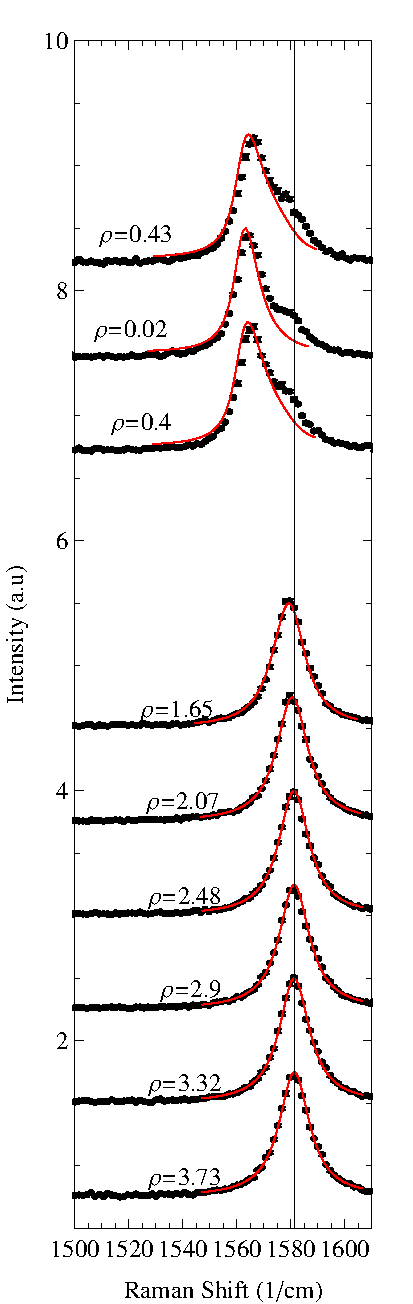
\includegraphics[scale=.675]{Figs_Fit/2012-12-18_Fit_101psi_Spectra_for_paper_sb04-6b.pdf}};
	
	%The picture of the hole
	\newcommand{\arrowlength}{.144*2.4 cm}%.144 is 2.5 um
	\begin{scope}[xshift=-.5 cm,yshift=1.25 cm]
		%For the total scale=1 the .jpg scale is .6
		\node at (0,0) {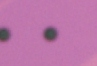
\includegraphics[scale=.30375,angle=-90]{Figs_Fit/SB04-6b.jpg}};%was .225 before I change the scale from .5 to .45
		\draw[->,black,>=stealth] (-.03cm,-\arrowlength-.05 cm-.136 cm) -- +(0,2*\arrowlength);
	\end{scope}
\end{tikzpicture}